\section{Il contenuto}
Dopo aver esaminato nel dettaglio la homepage, qua di seguito verranno analizzate le pagine interne più significative e alcuni aspetti comuni in esse, come breadcrumb e ricerca. 

\subsection{Intestazione}
Ogni pagina del sito, sia homepage che interna, ha la stessa intestazione, che consta del logo, del menù e soprattutto della barra di ricerca.
\begin{figure}[!htb]
	\center{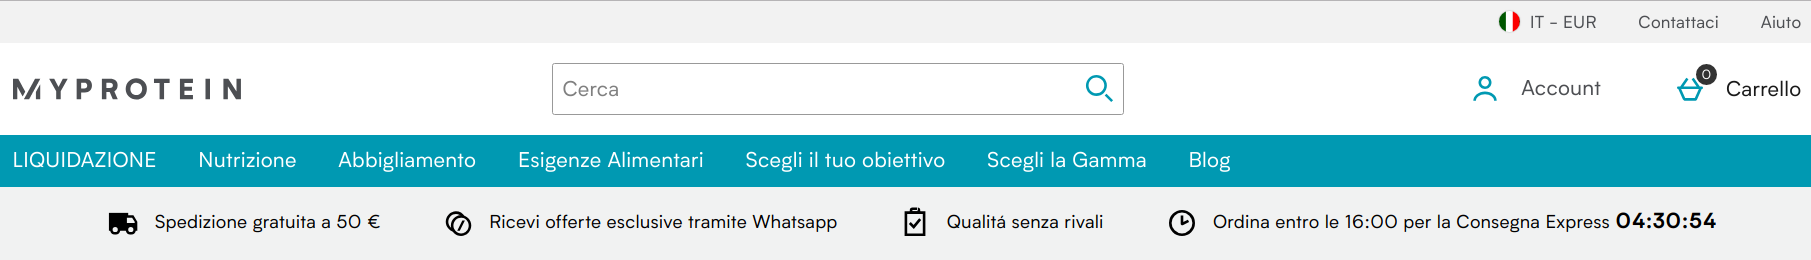
\includegraphics[width=\textwidth]
		{img/figura5.png}}
	\caption{\label{fig:figura5}} Intestazione del sito, comune a tutte le pagine.
\end{figure}


\subsection{Ricerca}
MyProtein offre centinaia di prodotti di eterogenee caratteristiche, che vanno dagl integratori ai capi di abbigliamento. E' quindi fondamentale la funzionalità di \textit{ricerca interna} che il sito offre. Essa è presente nella parte alta di tutte le pagine, ed è implementata con:
\begin{itemize}
    \item Un campo di testo, nel quale ci stanno circa 38 caratteri;
    \item Un tasto che scatena la ricerca, contenente l'icona della lente.
\end{itemize}
Le dimensioni del box di ricerca sono adeguate, considerando che la capienza minima consigliata è di circa 30 caratteri. Il tasto che scatena la ricerca, invece, ha solo l'icona della lente, senza testo. Anche se è stato dimostrato che gli utenti si trovano più a loro agio con la scritta "search" o "cerca", l'icona della lente è ormai una convenzione nel web. Finchè poi si scrive, il tasto si "evidenzia" colorandosi di bianco su sfondo blu, evidenziando il fatto che sia cliccabile, come visibile in figura 6. Inoltre, la ricerca può essere lanciata anche con il tasto "invio" della tastiera.\\
Sempre in figura 6 sono visibili i suggerimenti di ricerca, calcolati in tempo reale mentre l'utente scrive sul campo di ricerca, divisi in due tipologie:
\begin{itemize}
    \item completamento della query in base alle ricerche frequenti, nella parte superiore;
    \item prodotti più comuni suggeriti in base alla query scritta, nella parte inferiore.
\end{itemize}
Per selezionare un suggerimento si può usare il mouse (clicandoci sopra) o la tastiera (tramite le frecce direzionali e il tasto invio). Il menù a tendina in cui sono contenuti tali suggerimenti, inoltre, è fault tolerant, in quanto non si chiude se ci si sposta al di fuori di esso con il puntatore del mouse. \\
Personalmente trovo i prodotti più comuni nei suggerimenti di ricerca molto utili e, grazie ad essi, non vi è quasi mai il bisogno di utilizzare la pagina che mostra i risultati completi (che descriverò nella sezione successiva). La rappresentazione dei prodotti è scarna ma molto efficace: è presente il nome, una piccola immagine di anteprima (inutile ma graficamente piacevole), la valutazione media e, soprattutto, un'indicazione di prezzo.
\begin{figure}[!htb]
	\center{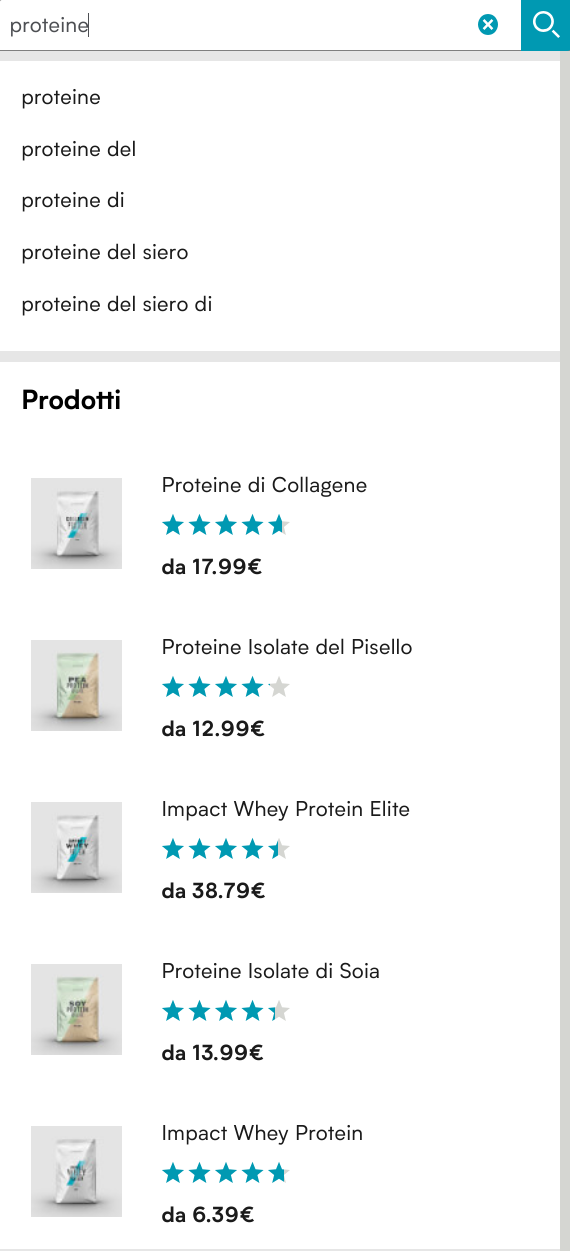
\includegraphics[width=0.5\textwidth]
		{img/figura6.png}}
	\caption{\label{fig:figura6}} Suggerimenti di ricerca.
\end{figure}

\subsection{Visualizzazzione risultati}